% Options for packages loaded elsewhere
\PassOptionsToPackage{unicode}{hyperref}
\PassOptionsToPackage{hyphens}{url}
\PassOptionsToPackage{dvipsnames,svgnames,x11names}{xcolor}
%
\documentclass[
  letterpaper,
  DIV=11,
  numbers=noendperiod]{scrreprt}

\usepackage{amsmath,amssymb}
\usepackage{iftex}
\ifPDFTeX
  \usepackage[T1]{fontenc}
  \usepackage[utf8]{inputenc}
  \usepackage{textcomp} % provide euro and other symbols
\else % if luatex or xetex
  \usepackage{unicode-math}
  \defaultfontfeatures{Scale=MatchLowercase}
  \defaultfontfeatures[\rmfamily]{Ligatures=TeX,Scale=1}
\fi
\usepackage{lmodern}
\ifPDFTeX\else  
    % xetex/luatex font selection
\fi
% Use upquote if available, for straight quotes in verbatim environments
\IfFileExists{upquote.sty}{\usepackage{upquote}}{}
\IfFileExists{microtype.sty}{% use microtype if available
  \usepackage[]{microtype}
  \UseMicrotypeSet[protrusion]{basicmath} % disable protrusion for tt fonts
}{}
\makeatletter
\@ifundefined{KOMAClassName}{% if non-KOMA class
  \IfFileExists{parskip.sty}{%
    \usepackage{parskip}
  }{% else
    \setlength{\parindent}{0pt}
    \setlength{\parskip}{6pt plus 2pt minus 1pt}}
}{% if KOMA class
  \KOMAoptions{parskip=half}}
\makeatother
\usepackage{xcolor}
\setlength{\emergencystretch}{3em} % prevent overfull lines
\setcounter{secnumdepth}{5}
% Make \paragraph and \subparagraph free-standing
\makeatletter
\ifx\paragraph\undefined\else
  \let\oldparagraph\paragraph
  \renewcommand{\paragraph}{
    \@ifstar
      \xxxParagraphStar
      \xxxParagraphNoStar
  }
  \newcommand{\xxxParagraphStar}[1]{\oldparagraph*{#1}\mbox{}}
  \newcommand{\xxxParagraphNoStar}[1]{\oldparagraph{#1}\mbox{}}
\fi
\ifx\subparagraph\undefined\else
  \let\oldsubparagraph\subparagraph
  \renewcommand{\subparagraph}{
    \@ifstar
      \xxxSubParagraphStar
      \xxxSubParagraphNoStar
  }
  \newcommand{\xxxSubParagraphStar}[1]{\oldsubparagraph*{#1}\mbox{}}
  \newcommand{\xxxSubParagraphNoStar}[1]{\oldsubparagraph{#1}\mbox{}}
\fi
\makeatother

\usepackage{color}
\usepackage{fancyvrb}
\newcommand{\VerbBar}{|}
\newcommand{\VERB}{\Verb[commandchars=\\\{\}]}
\DefineVerbatimEnvironment{Highlighting}{Verbatim}{commandchars=\\\{\}}
% Add ',fontsize=\small' for more characters per line
\usepackage{framed}
\definecolor{shadecolor}{RGB}{241,243,245}
\newenvironment{Shaded}{\begin{snugshade}}{\end{snugshade}}
\newcommand{\AlertTok}[1]{\textcolor[rgb]{0.68,0.00,0.00}{#1}}
\newcommand{\AnnotationTok}[1]{\textcolor[rgb]{0.37,0.37,0.37}{#1}}
\newcommand{\AttributeTok}[1]{\textcolor[rgb]{0.40,0.45,0.13}{#1}}
\newcommand{\BaseNTok}[1]{\textcolor[rgb]{0.68,0.00,0.00}{#1}}
\newcommand{\BuiltInTok}[1]{\textcolor[rgb]{0.00,0.23,0.31}{#1}}
\newcommand{\CharTok}[1]{\textcolor[rgb]{0.13,0.47,0.30}{#1}}
\newcommand{\CommentTok}[1]{\textcolor[rgb]{0.37,0.37,0.37}{#1}}
\newcommand{\CommentVarTok}[1]{\textcolor[rgb]{0.37,0.37,0.37}{\textit{#1}}}
\newcommand{\ConstantTok}[1]{\textcolor[rgb]{0.56,0.35,0.01}{#1}}
\newcommand{\ControlFlowTok}[1]{\textcolor[rgb]{0.00,0.23,0.31}{\textbf{#1}}}
\newcommand{\DataTypeTok}[1]{\textcolor[rgb]{0.68,0.00,0.00}{#1}}
\newcommand{\DecValTok}[1]{\textcolor[rgb]{0.68,0.00,0.00}{#1}}
\newcommand{\DocumentationTok}[1]{\textcolor[rgb]{0.37,0.37,0.37}{\textit{#1}}}
\newcommand{\ErrorTok}[1]{\textcolor[rgb]{0.68,0.00,0.00}{#1}}
\newcommand{\ExtensionTok}[1]{\textcolor[rgb]{0.00,0.23,0.31}{#1}}
\newcommand{\FloatTok}[1]{\textcolor[rgb]{0.68,0.00,0.00}{#1}}
\newcommand{\FunctionTok}[1]{\textcolor[rgb]{0.28,0.35,0.67}{#1}}
\newcommand{\ImportTok}[1]{\textcolor[rgb]{0.00,0.46,0.62}{#1}}
\newcommand{\InformationTok}[1]{\textcolor[rgb]{0.37,0.37,0.37}{#1}}
\newcommand{\KeywordTok}[1]{\textcolor[rgb]{0.00,0.23,0.31}{\textbf{#1}}}
\newcommand{\NormalTok}[1]{\textcolor[rgb]{0.00,0.23,0.31}{#1}}
\newcommand{\OperatorTok}[1]{\textcolor[rgb]{0.37,0.37,0.37}{#1}}
\newcommand{\OtherTok}[1]{\textcolor[rgb]{0.00,0.23,0.31}{#1}}
\newcommand{\PreprocessorTok}[1]{\textcolor[rgb]{0.68,0.00,0.00}{#1}}
\newcommand{\RegionMarkerTok}[1]{\textcolor[rgb]{0.00,0.23,0.31}{#1}}
\newcommand{\SpecialCharTok}[1]{\textcolor[rgb]{0.37,0.37,0.37}{#1}}
\newcommand{\SpecialStringTok}[1]{\textcolor[rgb]{0.13,0.47,0.30}{#1}}
\newcommand{\StringTok}[1]{\textcolor[rgb]{0.13,0.47,0.30}{#1}}
\newcommand{\VariableTok}[1]{\textcolor[rgb]{0.07,0.07,0.07}{#1}}
\newcommand{\VerbatimStringTok}[1]{\textcolor[rgb]{0.13,0.47,0.30}{#1}}
\newcommand{\WarningTok}[1]{\textcolor[rgb]{0.37,0.37,0.37}{\textit{#1}}}

\providecommand{\tightlist}{%
  \setlength{\itemsep}{0pt}\setlength{\parskip}{0pt}}\usepackage{longtable,booktabs,array}
\usepackage{calc} % for calculating minipage widths
% Correct order of tables after \paragraph or \subparagraph
\usepackage{etoolbox}
\makeatletter
\patchcmd\longtable{\par}{\if@noskipsec\mbox{}\fi\par}{}{}
\makeatother
% Allow footnotes in longtable head/foot
\IfFileExists{footnotehyper.sty}{\usepackage{footnotehyper}}{\usepackage{footnote}}
\makesavenoteenv{longtable}
\usepackage{graphicx}
\makeatletter
\def\maxwidth{\ifdim\Gin@nat@width>\linewidth\linewidth\else\Gin@nat@width\fi}
\def\maxheight{\ifdim\Gin@nat@height>\textheight\textheight\else\Gin@nat@height\fi}
\makeatother
% Scale images if necessary, so that they will not overflow the page
% margins by default, and it is still possible to overwrite the defaults
% using explicit options in \includegraphics[width, height, ...]{}
\setkeys{Gin}{width=\maxwidth,height=\maxheight,keepaspectratio}
% Set default figure placement to htbp
\makeatletter
\def\fps@figure{htbp}
\makeatother

\usepackage{cancel}
\KOMAoption{captions}{tableheading}
\makeatletter
\@ifpackageloaded{bookmark}{}{\usepackage{bookmark}}
\makeatother
\makeatletter
\@ifpackageloaded{caption}{}{\usepackage{caption}}
\AtBeginDocument{%
\ifdefined\contentsname
  \renewcommand*\contentsname{Table of contents}
\else
  \newcommand\contentsname{Table of contents}
\fi
\ifdefined\listfigurename
  \renewcommand*\listfigurename{List of Figures}
\else
  \newcommand\listfigurename{List of Figures}
\fi
\ifdefined\listtablename
  \renewcommand*\listtablename{List of Tables}
\else
  \newcommand\listtablename{List of Tables}
\fi
\ifdefined\figurename
  \renewcommand*\figurename{Figure}
\else
  \newcommand\figurename{Figure}
\fi
\ifdefined\tablename
  \renewcommand*\tablename{Table}
\else
  \newcommand\tablename{Table}
\fi
}
\@ifpackageloaded{float}{}{\usepackage{float}}
\floatstyle{ruled}
\@ifundefined{c@chapter}{\newfloat{codelisting}{h}{lop}}{\newfloat{codelisting}{h}{lop}[chapter]}
\floatname{codelisting}{Listing}
\newcommand*\listoflistings{\listof{codelisting}{List of Listings}}
\makeatother
\makeatletter
\makeatother
\makeatletter
\@ifpackageloaded{caption}{}{\usepackage{caption}}
\@ifpackageloaded{subcaption}{}{\usepackage{subcaption}}
\makeatother

\ifLuaTeX
  \usepackage{selnolig}  % disable illegal ligatures
\fi
\usepackage{bookmark}

\IfFileExists{xurl.sty}{\usepackage{xurl}}{} % add URL line breaks if available
\urlstyle{same} % disable monospaced font for URLs
\hypersetup{
  pdftitle={Time Series Analysis},
  pdfauthor={Yair Mau},
  colorlinks=true,
  linkcolor={blue},
  filecolor={Maroon},
  citecolor={Blue},
  urlcolor={Blue},
  pdfcreator={LaTeX via pandoc}}


\title{Time Series Analysis}
\author{Yair Mau}
\date{}

\begin{document}
\maketitle

\renewcommand*\contentsname{Table of contents}
{
\hypersetup{linkcolor=}
\setcounter{tocdepth}{2}
\tableofcontents
}

\bookmarksetup{startatroot}

\chapter*{about}\label{about}
\addcontentsline{toc}{chapter}{about}

\markboth{about}{about}

Welcome to \textbf{Time Series Analysis for Environmental Sciences}
(71106) at the Hebrew University of Jerusalem. This is Yair Mau, your
host for today. I am a senior lecturer at the Institute of Environmental
Sciences, at the Faculty of Agriculture, Food and Environment, in
Rehovot, Israel.

This website contains (almost) all the material you'll need for the
course. If you find any mistakes, or have any comments, please email me.

\section*{disclaimer}\label{disclaimer}
\addcontentsline{toc}{section}{disclaimer}

\markright{disclaimer}

The material here is not comprehensive and \texttt{does\ not} constitute
a stand alone course in Time Series Analysis. This is only the support
material for the actual presential course I give.

\section*{what, who, when and where?}\label{what-who-when-and-where}
\addcontentsline{toc}{section}{what, who, when and where?}

\markright{what, who, when and where?}

Course number 71106, 3 academic points\\
Yair Mau (lecturer), Erez Feuer (TA)\\
Tuesdays, from 11:15 to 14:00\\
Computer \href{https://goo.gl/maps/rzniv9NuyEs4ETH58}{classroom \#18}\\
Office hours: Tuesdays, from 09:45 to 10:45 (you should send an email to
let me know you are coming)

\section*{syllabus}\label{syllabus}
\addcontentsline{toc}{section}{syllabus}

\markright{syllabus}

\subsection*{course description}\label{course-description}
\addcontentsline{toc}{subsection}{course description}

Data analysis of time series, with practical examples from environmental
sciences.

\subsection*{course aims}\label{course-aims}
\addcontentsline{toc}{subsection}{course aims}

This course aims at giving the students a broad overview of the main
steps involved in the analysis of time series: data management, data
wrangling, visualization, analysis, and forecast. The course will
provide a hands-on approach, where students will actively engage with
real-life datasets from the field of environmental science.

\subsection*{learning outcomes}\label{learning-outcomes}
\addcontentsline{toc}{subsection}{learning outcomes}

On successful completion of this module,students should be able to:

\begin{itemize}
\tightlist
\item
  Explore a time-series dataset, while formulating interesting
  questions.
\item
  Choose the appropriate tools to attack the problem and answer the
  questions.
\item
  Communicate their findings and the methods they used to achieve them,
  using graphs, statistics, text, and a well-documented code.
\end{itemize}

\subsection*{course content}\label{course-content}
\addcontentsline{toc}{subsection}{course content}

\begin{itemize}
\tightlist
\item
  \textbf{Data wrangling:} organization, cleaning, merging, filling
  gaps, excluding outliers, smoothing, resampling.
\item
  \textbf{Visualization:} best practices for graph making using leading
  python libraries.
\item
  \textbf{Analysis:} stationarity, seasonality, (auto)correlations,
  lags, derivatives, spectral analysis.
\item
  \textbf{Forecast:} ARIMA
\item
  \textbf{Data management:} how to plan ahead and best organize large
  quantities of data. If there is enough time, we will build a simple
  time-series database.
\end{itemize}

\subsection*{books and other sources}\label{books-and-other-sources}
\addcontentsline{toc}{subsection}{books and other sources}

\href{references.html}{Click here.}

\subsection*{course evaluation}\label{course-evaluation}
\addcontentsline{toc}{subsection}{course evaluation}

There will be assignments during the semester (totaling 50\% of the
final grade), and one final project (50\%).

\subsection*{Evaluation policy}\label{evaluation-policy}
\addcontentsline{toc}{subsection}{Evaluation policy}

\begin{itemize}
\item
  \textbf{Individual Work:} While we support helping your peers, it's
  important to remember that all assignments must be completed
  individually. This means that your submissions should be your own
  unique work and not contain code or text that is identical to someone
  else's.
\item
  \textbf{Zero Plagiarism:} Do not copy text verbatim from any source.
  Always express ideas in your own words.
\item
  \textbf{On-Time Submission:} Assignments must be turned in by the
  specified deadline. Late submissions will receive a grade of 0. If you
  require an extension, requests will only be considered if made at
  least 24 hours before the due date.
\item
  \textbf{Non-Compliance Consequence:} Assignments that do not adhere to
  these guidelines will automatically receive a grade of 0.
\end{itemize}

\bookmarksetup{startatroot}

\chapter*{2024/2025 Schedule}\label{schedule}
\addcontentsline{toc}{chapter}{2024/2025 Schedule}

\markboth{2024/2025 Schedule}{2024/2025 Schedule}

\subsection*{Week 1, 29 Oct 2024}\label{week-1-29-oct-2024}
\addcontentsline{toc}{subsection}{Week 1, 29 Oct 2024}

\textbf{Introduction}

Course overview, setting of expectations, introduction to Jupyter
Notebooks, loading data and plotting it.

\href{assignments/assignment1}{Assignment 1}, due 12 Nov 2024

\subsection*{Week 2, 5 Nov 2024}\label{week-2-5-nov-2024}
\addcontentsline{toc}{subsection}{Week 2, 5 Nov 2024}

Resampling

\subsection*{Week 3, 12 Nov 2024}\label{week-3-12-nov-2024}
\addcontentsline{toc}{subsection}{Week 3, 12 Nov 2024}

Smoothing

\href{assignments/assignment2}{Assignment 2}, due 26 Nov 2024

\subsection*{Week 4, 19 Nov 2024}\label{week-4-19-nov-2024}
\addcontentsline{toc}{subsection}{Week 4, 19 Nov 2024}

Outliers

\subsection*{Week 5, 26 Nov 2024}\label{week-5-26-nov-2024}
\addcontentsline{toc}{subsection}{Week 5, 26 Nov 2024}

Stationarity: random processes, statistics refresher, AR processes

\href{assignments/assignment3}{Assignment 3}, due 10 Dec 2024

\subsection*{Week 6, 3 Dec 2024}\label{week-6-3-dec-2024}
\addcontentsline{toc}{subsection}{Week 6, 3 Dec 2024}

Stationarity: ACF and PACF graphs

\subsection*{Week 7, 10 Dec 2024}\label{week-7-10-dec-2024}
\addcontentsline{toc}{subsection}{Week 7, 10 Dec 2024}

Stationarity: Forecasting, ARIMA, SARIMA, SARIMAX

\href{assignments/assignment4}{Assignment 4}, due 31 Dec 2024

\subsection*{Week 8, 17 Dec 2024}\label{week-8-17-dec-2024}
\addcontentsline{toc}{subsection}{Week 8, 17 Dec 2024}

Seasonality

\subsection*{24 Dec 2024}\label{dec-2024}
\addcontentsline{toc}{subsection}{24 Dec 2024}

{No classes.}

\subsection*{Week 9, 31 Dec 2024}\label{week-9-31-dec-2024}
\addcontentsline{toc}{subsection}{Week 9, 31 Dec 2024}

\href{assignments/assignment5}{Assignment 5}, due 14 Jan 2025

\subsection*{Week 10, 7 Jan 2025}\label{week-10-7-jan-2025}
\addcontentsline{toc}{subsection}{Week 10, 7 Jan 2025}

\subsection*{Week 11, 14 Jan 2025}\label{week-11-14-jan-2025}
\addcontentsline{toc}{subsection}{Week 11, 14 Jan 2025}

\href{assignments/assignment6}{Assignment 6}, due 28 Jan 2025

\subsection*{Week 12, 21 Jan 2025}\label{week-12-21-jan-2025}
\addcontentsline{toc}{subsection}{Week 12, 21 Jan 2025}

\subsection*{Week 13, 28 Jan 2025}\label{week-13-28-jan-2025}
\addcontentsline{toc}{subsection}{Week 13, 28 Jan 2025}

\href{assignments/final-project}{Final project}, due 4 Mar 2025

\bookmarksetup{startatroot}

\chapter*{who cares?}\label{who-cares}
\addcontentsline{toc}{chapter}{who cares?}

\markboth{who cares?}{who cares?}

\section*{why ``Time Series Analysis?''}\label{why-time-series-analysis}
\addcontentsline{toc}{section}{why ``Time Series Analysis?''}

\markright{why ``Time Series Analysis?''}

Time has two aspects. There is the arrow, the running river, without
which there is no change, no progress, or direction, or creation. And
there is the circle or the cycle, without which there is chaos,
meaningless succession of instants, a world without clocks or seasons or
promises.\\
URSULA K. LE GUIN

You are here because you are interested in how things change, evolve. In
this course I want to discuss with you how to make sense of data whose
temporal nature is in its very essence. We will talk about randomness,
cycles, frequencies, correlations, and more.

\section*{why ``Environmental
Sciences''}\label{why-environmental-sciences}
\addcontentsline{toc}{section}{why ``Environmental Sciences''}

\markright{why ``Environmental Sciences''}

This same time series analysis (TSA) course could be called instead
``TSA for finance'', ``TSA for Biology'', or any other application. The
emphasis in this course is \textbf{not} Environmental Sciences, but the
concepts and tools of TSA. Because my research is in Environmental
Science, and many of the graduate students at HUJI-Rehovot research
this, I chose to use examples ``close to home''. The same toolset should
be useful for students of other disciplines.

\section*{what is it good for?}\label{what-is-it-good-for}
\addcontentsline{toc}{section}{what is it good for?}

\markright{what is it good for?}

In many fields of science we are flooded by data, and it's hard to see
the forest for the trees. I hope that the topics we'll discuss in this
course can help you find meaningful patterns in your data, formulate
interesting hypotheses, and design better experiments.

\section*{do I need it?}\label{do-i-need-it}
\addcontentsline{toc}{section}{do I need it?}

\markright{do I need it?}

Maybe. If you are a grad student and you have temporal data to analyze,
then probably yes. However, I have very fond memories of courses that I
took as a grad student that were completely unrelated to my research.
Sometimes ``because it's fun'' is a perfectly good answer.

\section*{\texorpdfstring{what will I \textbf{actually} gain from
it?}{what will I actually gain from it?}}\label{what-will-i-actually-gain-from-it}
\addcontentsline{toc}{section}{what will I \textbf{actually} gain from
it?}

\markright{what will I \textbf{actually} gain from it?}

By the end of this course you will have gained:

\begin{itemize}
\tightlist
\item
  a \textbf{hands-on} experience of fundamental time-series analysis
  tools
\item
  an \textbf{intuition} regarding the basic concepts
\item
  \textbf{technical} abilities
\item
  a \textbf{springboard} for learning more about the subject by yourself
\end{itemize}

\part{start here}

\chapter{the boring stuff you absolutely need to
do}\label{the-boring-stuff-you-absolutely-need-to-do}

I assume everyone registered has taken a basic Python course. On your
computer, do the following:

\section{Anaconda}\label{anaconda}

Install \href{https://www.anaconda.com/download}{Anaconda's Python
distribution}. The Anaconda installation brings with it all the main
python packages we will need to use. In order to install extra packages,
refer to these two tutorials:
\href{https://www.tutorialspoint.com/how-do-i-install-python-packages-in-anaconda}{tutorial
1},
\href{https://docs.anaconda.com/free/anaconda/packages/install-packages.html}{tutorial
2}.

\section{VSCode}\label{vscode}

Install \href{https://code.visualstudio.com/download}{VSCode}. Visual
Studio Code is a very nice IDE (Integrated Development Environment) made
by Microsoft, available to all operating systems. Contrary to the title
of this page, it is not absolutely necessary to use it, but I like
VSCode, and as my student, so do you 😉.

\section{jupyter notebooks}\label{jupyter-notebooks}

We will code exclusively in Jupyter Notebooks.
\href{https://code.visualstudio.com/docs/datascience/jupyter-notebooks}{Get
acquainted with them}. Make sure you can
\href{https://opensourceoptions.com/blog/setup-anaconda-python-to-work-with-visual-studio-code-on-windows/}{point
VSCode} to the Anaconda environment of your choice (``base'' by
default). Don't worry, this is easier than it sounds.

One failproof way of making sure VSCode uses the Anaconda installation
is the following:

\begin{itemize}
\tightlist
\item
  Open Anaconda Navigator
\item
  If you are using HUJI's computers, in ``Environments'', choose
  ``asgard''. If you are using your own computer, ignore this step.
\item
  open VSCode from inside Anaconda Navigator (see image below).
\end{itemize}

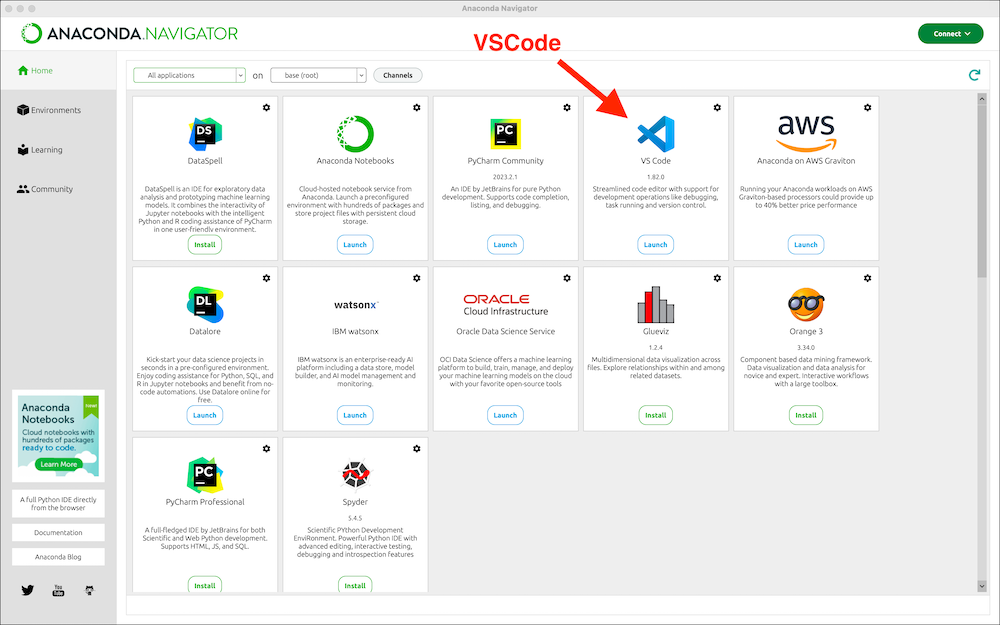
\includegraphics{basics/anacondanavigator.png}

Sometimes you will need to manualy install the Jupyter extension on
VSCode. In this case follow
\href{https://code.visualstudio.com/docs/datascience/jupyter-notebooks}{this
tutorial}.

\section{folder structure}\label{folder-structure}

You \textbf{NEED} to be confortable with you computer's folder (or
directory) structure. Where are files located? How to navigate through
different folders? How is my stuff organized? If you don't feel
\textbf{absolutely} comfortable with this, then read this,
\href{http://www2.westsussex.gov.uk/LearningandDevelopment/IT\%20Learning\%20Guides/Microsoft\%20Windows\%207/05\%20Working\%20with\%20folders.pdf}{Windows},
\href{https://recoverit.wondershare.com/mac-tips/mac-finder-tutorial-mac.html}{MacOS}.
If you use Linux then you surely know this stuff. \textbf{Make yourself
a ``time-series'' folder} wherever you want, and have it backed up
regularly (use Google Drive, Dropbox, do it manually, etc). ``My dog
deleted my files'' is not an excuse.

\chapter{numpy, pandas, matplotlib}\label{numpy-pandas-matplotlib}

\begin{Shaded}
\begin{Highlighting}[]
\ImportTok{import}\NormalTok{ numpy }\ImportTok{as}\NormalTok{ np}
\ImportTok{import}\NormalTok{ pandas }\ImportTok{as}\NormalTok{ pd}
\ImportTok{import}\NormalTok{ matplotlib.pyplot }\ImportTok{as}\NormalTok{ plt}
\end{Highlighting}
\end{Shaded}

The three lines above are the most common way you will start every
project in this course.

\begin{itemize}
\tightlist
\item
  \textbf{numpy} = numerical python. This library has a ton useful
  mathematical functions, and most importantly, it has an object called
  \texttt{numpy\ array}, which is one of the most useful data structures
  we have for time series analysis.
\item
  \textbf{pandas} is built upon numpy, and allows us to easily
  manipulate data stored in \texttt{dataframes}, a fancy name for a
  table.
\item
  \textbf{pyplot} is a submodule of \texttt{matplotlib}, and allows us
  to beautifully plot data.
\end{itemize}

The best resource I know to get acquainted with all three packages is
\href{https://jakevdp.github.io/PythonDataScienceHandbook/index.html}{Python
Data Science Handbook, by Jake VanderPlas}. This is a free online book,
with excellent step by step examples.

\section{pandas}\label{pandas}

We will primarily use the Pandas package to deal with data. Pandas has
become the standard Python tool to manipulate time series, and you
should get acquainted with its basic usage. This course will provide you
the opportunity to learn by example, but I'm sure we will only scratch
the surface, and you'll be left with lots of questions.

I provide below a (non-comprehensive) list of useful tutorials, they are
a good reference for the beginner and for the experienced user.

\begin{itemize}
\tightlist
\item
  \href{https://jakevdp.github.io/PythonDataScienceHandbook/index.html}{Python
  Data Science Handbook, by Jake VanderPlas}
\item
  \href{https://pandas.pydata.org/Pandas_Cheat_Sheet.pdf}{Data Wrangling
  with pandas Cheat Sheet}
\item
  \href{https://images.datacamp.com/image/upload/v1666944896/Marketing/Blog/Working_with_Dates_and_Times_Cheat_Sheet.pdf}{Working
  with Dates and Times in Python}
\item
  \href{https://www.webpages.uidaho.edu/~stevel/cheatsheets/Pandas\%20DataFrame\%20Notes_12pages.pdf}{Cheat
  Sheet: The pandas DataFrame Object}
\item
  \href{https://www.youtube.com/watch?v=ZyhVh-qRZPA&list=PL-osiE80TeTsWmV9i9c58mdDCSskIFdDS&pp=iAQB}{YouTube
  tutorials} by Corey Schafer
\end{itemize}

\section{pyplot}\label{pyplot}

Matplotlib, and its submodule pyplot, are probably the most common
Python plotting tool. Pyplot is both great and horrible:

\begin{itemize}
\tightlist
\item
  Great: you'll have absolutely full control of everything you want to
  plot. The sky is the limit.
\item
  Horrible: you'll cry as you do it, because there is so much to know,
  and it is not the most friendly plotting package.
\end{itemize}

Pyplot is \emph{object oriented}, so you will usually manipulate the
\textbf{axes} object like this.

\begin{Shaded}
\begin{Highlighting}[]
\ImportTok{import}\NormalTok{ matplotlib.pyplot }\ImportTok{as}\NormalTok{ plt}

\NormalTok{x }\OperatorTok{=}\NormalTok{ [}\DecValTok{1}\NormalTok{, }\DecValTok{2}\NormalTok{, }\DecValTok{3}\NormalTok{, }\DecValTok{4}\NormalTok{, }\DecValTok{5}\NormalTok{]}
\NormalTok{y }\OperatorTok{=}\NormalTok{ [}\DecValTok{1}\NormalTok{, }\DecValTok{4}\NormalTok{, }\DecValTok{2}\NormalTok{, }\DecValTok{0}\NormalTok{, }\DecValTok{3}\NormalTok{]}

\CommentTok{\# Figure with two plots}
\NormalTok{fig, (ax1, ax2) }\OperatorTok{=}\NormalTok{ plt.subplots(}\DecValTok{1}\NormalTok{, }\DecValTok{2}\NormalTok{, figsize }\OperatorTok{=}\NormalTok{ (}\DecValTok{8}\NormalTok{, }\DecValTok{6}\NormalTok{))}
\CommentTok{\# plot on the left}
\NormalTok{ax1.plot(x, y, color}\OperatorTok{=}\StringTok{"tab:blue"}\NormalTok{)}
\NormalTok{ax1.plot(x, y[::}\OperatorTok{{-}}\DecValTok{1}\NormalTok{], color}\OperatorTok{=}\StringTok{"tab:orange"}\NormalTok{)}
\NormalTok{ax1.}\BuiltInTok{set}\NormalTok{(xlabel}\OperatorTok{=}\StringTok{"date"}\NormalTok{,}
\NormalTok{        ylabel}\OperatorTok{=}\StringTok{"something"}\NormalTok{,}
\NormalTok{        title}\OperatorTok{=}\StringTok{"left panel"}\NormalTok{)}
\CommentTok{\# plot on the right}
\NormalTok{ax2.plot(x, y[::}\OperatorTok{{-}}\DecValTok{1}\NormalTok{])}
\NormalTok{ax2.}\BuiltInTok{set}\NormalTok{(xlabel}\OperatorTok{=}\StringTok{"date"}\NormalTok{,}
\NormalTok{        ylabel}\OperatorTok{=}\StringTok{"something else"}\NormalTok{,}
\NormalTok{        title}\OperatorTok{=}\StringTok{"right panel"}\NormalTok{)}
\end{Highlighting}
\end{Shaded}

\begin{verbatim}
[Text(0.5, 0, 'date'),
 Text(0, 0.5, 'something else'),
 Text(0.5, 1.0, 'right panel')]
\end{verbatim}

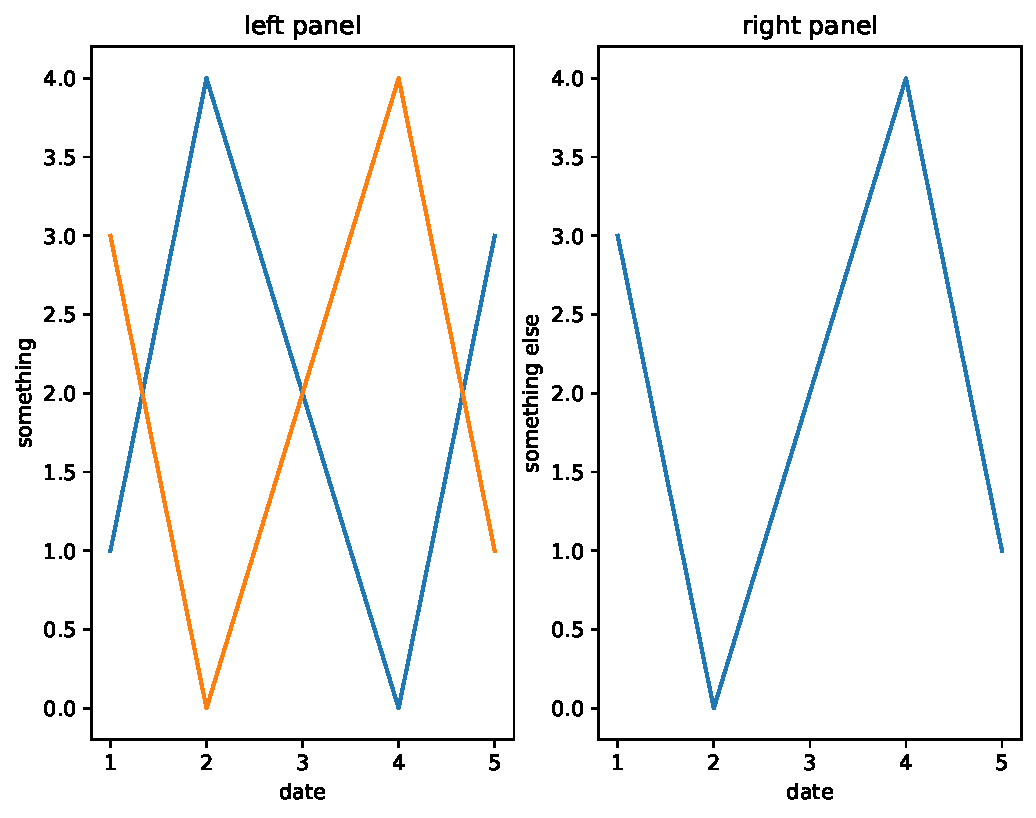
\includegraphics{basics/numpy-pandas-matplotlib_files/figure-pdf/cell-2-output-2.pdf}

For the very beginners, you need to know that \texttt{figure} refers to
the whole white canvas, and \texttt{axes} means the rectangle inside
which something will be plotted:

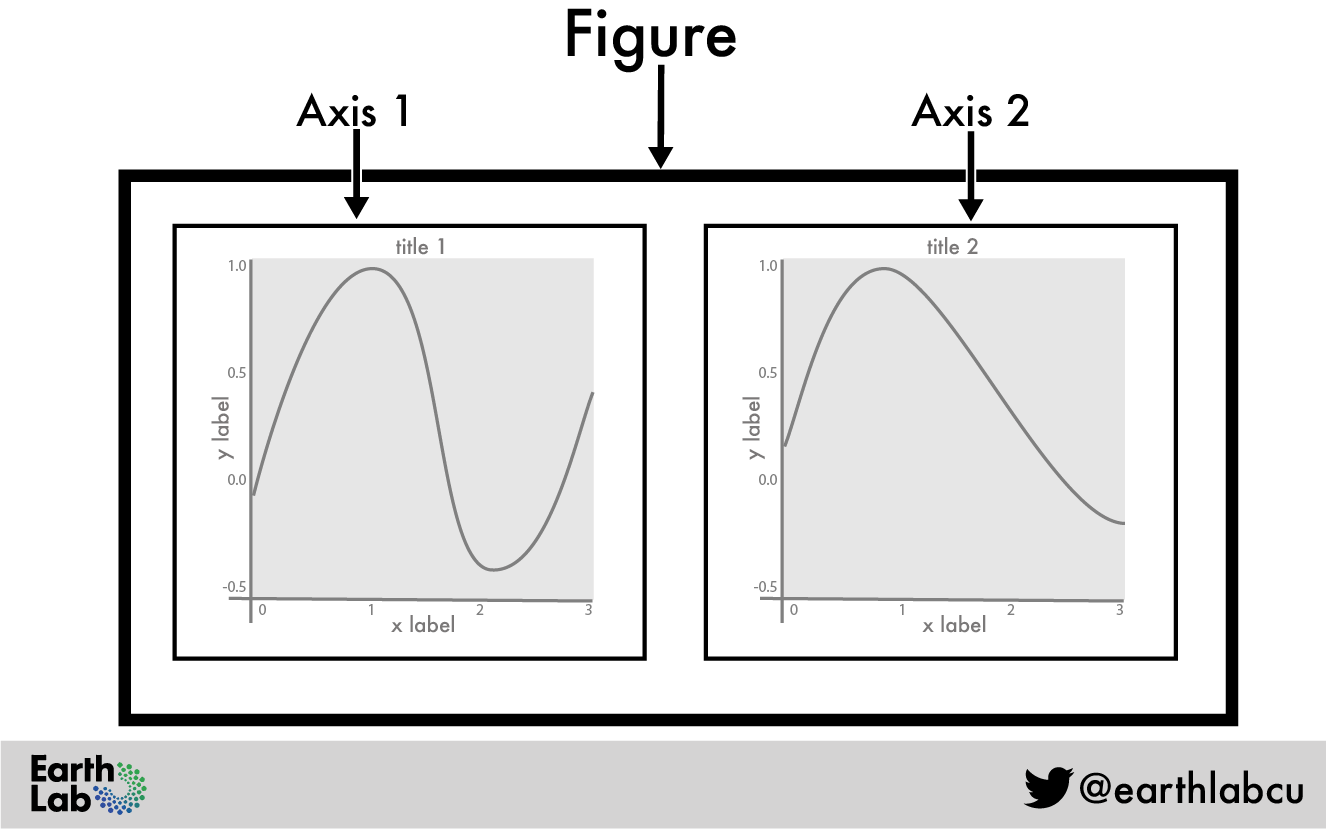
\includegraphics{basics/fig-2-plots.png}

The image above is good because it has 2 panels, and it's easy to
understand what going on. Sadly, they mixed the two terms, axis and
axes.

\begin{itemize}
\tightlist
\item
  \textbf{axes} is where the whole plot will be drawn. In the figure
  above it is the same as each panel.
\item
  \textbf{axis} is each of the vertical and horizontal lines, where you
  have ticks and numbers.
\end{itemize}

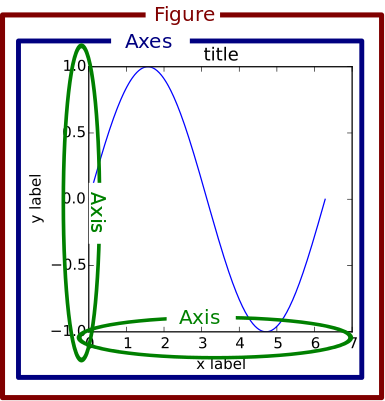
\includegraphics{basics/axis-vs-axes.png}

If you are new to all this, I recommend that you go to:

\begin{itemize}
\tightlist
\item
  \href{https://www.earthdatascience.org/courses/scientists-guide-to-plotting-data-in-python/plot-with-matplotlib/introduction-to-matplotlib-plots/}{Earth
  Lab's Introduction to Plotting in Python Using Matplotlib}
\item
  \href{https://jakevdp.github.io/PythonDataScienceHandbook/index.html}{Jake
  VanderPlas's Python Data Science Handbook}
\end{itemize}

\chapter{learn by example}\label{learn-by-example}

Now that everything is installed, try to run the code below
\emph{before} the first lecture. Don't worry if you don't understand
everything.

\begin{itemize}
\tightlist
\item
  If you manage to run everything without errors, this means that your
  computer is good to go!
\item
  You might encounter a few problems. That's ok. Make a note and we will
  solve everything in the first lecture.
\end{itemize}

Let's make a first plot of real data. We will use NOAA's Global
Monitoring Laboratory data on
\href{https://gml.noaa.gov/ccgg/trends/data.html}{Trends in Atmospheric
Carbon Dioxide}.

\section{open a new Jupyter Notebook}\label{open-a-new-jupyter-notebook}

\begin{enumerate}
\def\labelenumi{\arabic{enumi}.}
\tightlist
\item
  On your computer, open the program \texttt{Anaconda\ Navigator} (it
  may take a while to load).
\item
  Find the white box called \texttt{VS\ Code} and click \texttt{Launch}.
\item
  Now go to \texttt{File} \textgreater{} \texttt{Open\ Folder}, and open
  the folder you created for this course. VS Code may ask you if you
  trust the authors, and the answer is ``yes'' (it's your computer).
\item
  \texttt{File} \textgreater{} \texttt{New\ File}, and call it
  \texttt{example.ipynb}
\item
  You can start copying and pasting code from this website to your
  Jupyter Notebook. To run a cell, press Shift+Enter.
\item
  You may be asked to choose to Select Kernel. This is VS Code wanting
  to know which python installation to use. Click on ``Python
  Environments'', and then choose the option with the word
  \texttt{anaconda} in it.
\item
  That's all! Congratulations!
\end{enumerate}

\section{import packages}\label{import-packages}

First, import packages to be used. They should all be already included
in the Anaconda distribution you installed.

\begin{Shaded}
\begin{Highlighting}[]
\ImportTok{import}\NormalTok{ numpy }\ImportTok{as}\NormalTok{ np}
\ImportTok{import}\NormalTok{ matplotlib.pyplot }\ImportTok{as}\NormalTok{ plt}
\ImportTok{import}\NormalTok{ pandas }\ImportTok{as}\NormalTok{ pd}
\ImportTok{import}\NormalTok{ seaborn }\ImportTok{as}\NormalTok{ sns}
\NormalTok{sns.}\BuiltInTok{set}\NormalTok{(style}\OperatorTok{=}\StringTok{"ticks"}\NormalTok{, font\_scale}\OperatorTok{=}\FloatTok{1.5}\NormalTok{)  }\CommentTok{\# white graphs, with large and legible letters}
\end{Highlighting}
\end{Shaded}

\section{load data}\label{load-data}

Load CO2 data into a Pandas dataframe. You can load it directly from the
URL (option 1), or first download the CSV to your computer and then load
it (option 2). The link to download the data directly form NOAA is
\href{https://gml.noaa.gov/webdata/ccgg/trends/co2/co2_weekly_mlo.csv}{this}.
If for some reason this doesn't work, download here.

\begin{Shaded}
\begin{Highlighting}[]
\CommentTok{\# option 1: load data directly from URL}
\CommentTok{\# url = "https://gml.noaa.gov/webdata/ccgg/trends/co2/co2\_weekly\_mlo.csv"}
\CommentTok{\# df = pd.read\_csv(url,}
\CommentTok{\#                  header=34,}
\CommentTok{\#                  na\_values=[{-}999.99]}
\CommentTok{\#                  )}

\CommentTok{\# option 2: download first (use the URL above and save it to your computer), then load csv}
\NormalTok{filename }\OperatorTok{=} \StringTok{"co2\_weekly\_mlo.csv"}
\NormalTok{df }\OperatorTok{=}\NormalTok{ pd.read\_csv(filename,}
\NormalTok{                comment}\OperatorTok{=}\StringTok{\textquotesingle{}\#\textquotesingle{}}\NormalTok{,  }\CommentTok{\# will ignore rows starting with \#}
\NormalTok{                 na\_values}\OperatorTok{=}\NormalTok{[}\OperatorTok{{-}}\FloatTok{999.99}\NormalTok{]  }\CommentTok{\# substitute {-}999.99 for NaN (Not a Number), data not available}
\NormalTok{                 )}
\CommentTok{\# check how the dataframe (table) looks like}
\NormalTok{df}
\end{Highlighting}
\end{Shaded}

\begin{longtable}[]{@{}llllllllll@{}}
\toprule\noalign{}
& year & month & day & decimal & average & ndays & 1 year ago & 10 years
ago & increase since 1800 \\
\midrule\noalign{}
\endhead
\bottomrule\noalign{}
\endlastfoot
0 & 1974 & 5 & 19 & 1974.3795 & 333.37 & 5 & NaN & NaN & 50.39 \\
1 & 1974 & 5 & 26 & 1974.3986 & 332.95 & 6 & NaN & NaN & 50.05 \\
2 & 1974 & 6 & 2 & 1974.4178 & 332.35 & 5 & NaN & NaN & 49.59 \\
3 & 1974 & 6 & 9 & 1974.4370 & 332.20 & 7 & NaN & NaN & 49.64 \\
4 & 1974 & 6 & 16 & 1974.4562 & 332.37 & 7 & NaN & NaN & 50.06 \\
... & ... & ... & ... & ... & ... & ... & ... & ... & ... \\
2566 & 2023 & 7 & 23 & 2023.5575 & 421.28 & 4 & 418.03 & 397.30 &
141.60 \\
2567 & 2023 & 7 & 30 & 2023.5767 & 420.83 & 6 & 418.10 & 396.80 &
141.69 \\
2568 & 2023 & 8 & 6 & 2023.5959 & 420.02 & 6 & 417.36 & 395.65 &
141.41 \\
2569 & 2023 & 8 & 13 & 2023.6151 & 418.98 & 4 & 417.25 & 395.24 &
140.89 \\
2570 & 2023 & 8 & 20 & 2023.6342 & 419.31 & 2 & 416.64 & 395.22 &
141.71 \\
\end{longtable}

\section{dealing with dates}\label{dealing-with-dates}

Create a new column called \texttt{date}, that combines the information
from three separate columns: \texttt{year}, \texttt{month},
\texttt{day}.

\begin{Shaded}
\begin{Highlighting}[]
\CommentTok{\# function to\_datetime translates the full date into a pandas datetime object,}
\CommentTok{\# that is, pandas knows this is a date, it\textquotesingle{}s not just a string}
\NormalTok{df[}\StringTok{\textquotesingle{}date\textquotesingle{}}\NormalTok{] }\OperatorTok{=}\NormalTok{ pd.to\_datetime(df[[}\StringTok{\textquotesingle{}year\textquotesingle{}}\NormalTok{, }\StringTok{\textquotesingle{}month\textquotesingle{}}\NormalTok{, }\StringTok{\textquotesingle{}day\textquotesingle{}}\NormalTok{]])}
\CommentTok{\# make \textquotesingle{}date\textquotesingle{} column the dataframe index}
\NormalTok{df }\OperatorTok{=}\NormalTok{ df.set\_index(}\StringTok{\textquotesingle{}date\textquotesingle{}}\NormalTok{)}
\CommentTok{\# now see if everything is ok}
\NormalTok{df}
\end{Highlighting}
\end{Shaded}

\begin{longtable}[]{@{}llllllllll@{}}
\toprule\noalign{}
& year & month & day & decimal & average & ndays & 1 year ago & 10 years
ago & increase since 1800 \\
date & & & & & & & & & \\
\midrule\noalign{}
\endhead
\bottomrule\noalign{}
\endlastfoot
1974-05-19 & 1974 & 5 & 19 & 1974.3795 & 333.37 & 5 & NaN & NaN &
50.39 \\
1974-05-26 & 1974 & 5 & 26 & 1974.3986 & 332.95 & 6 & NaN & NaN &
50.05 \\
1974-06-02 & 1974 & 6 & 2 & 1974.4178 & 332.35 & 5 & NaN & NaN &
49.59 \\
1974-06-09 & 1974 & 6 & 9 & 1974.4370 & 332.20 & 7 & NaN & NaN &
49.64 \\
1974-06-16 & 1974 & 6 & 16 & 1974.4562 & 332.37 & 7 & NaN & NaN &
50.06 \\
... & ... & ... & ... & ... & ... & ... & ... & ... & ... \\
2023-07-23 & 2023 & 7 & 23 & 2023.5575 & 421.28 & 4 & 418.03 & 397.30 &
141.60 \\
2023-07-30 & 2023 & 7 & 30 & 2023.5767 & 420.83 & 6 & 418.10 & 396.80 &
141.69 \\
2023-08-06 & 2023 & 8 & 6 & 2023.5959 & 420.02 & 6 & 417.36 & 395.65 &
141.41 \\
2023-08-13 & 2023 & 8 & 13 & 2023.6151 & 418.98 & 4 & 417.25 & 395.24 &
140.89 \\
2023-08-20 & 2023 & 8 & 20 & 2023.6342 & 419.31 & 2 & 416.64 & 395.22 &
141.71 \\
\end{longtable}

\section{first plot}\label{first-plot}

We are now ready for our first plot! Let's see the weekly CO2 average.

\begin{Shaded}
\begin{Highlighting}[]
\CommentTok{\# \%matplotlib widget}
\CommentTok{\# uncomment the above line if you want dynamic control of the figure when using VSCode}
\NormalTok{fig, (ax1, ax2) }\OperatorTok{=}\NormalTok{ plt.subplots(}\DecValTok{1}\NormalTok{, }\DecValTok{2}\NormalTok{,  }\CommentTok{\# 1 row, 2 columns}
\NormalTok{                               figsize}\OperatorTok{=}\NormalTok{(}\DecValTok{8}\NormalTok{,}\DecValTok{5}\NormalTok{)  }\CommentTok{\# width, height, in inches}
\NormalTok{                               )}
\CommentTok{\# left panel}
\NormalTok{ax1.plot(df[}\StringTok{\textquotesingle{}average\textquotesingle{}}\NormalTok{], color}\OperatorTok{=}\StringTok{"black"}\NormalTok{)}
\NormalTok{ax1.plot(df.loc[}\StringTok{\textquotesingle{}2010{-}01{-}01\textquotesingle{}}\NormalTok{:}\StringTok{\textquotesingle{}2011{-}12{-}31\textquotesingle{}}\NormalTok{,}\StringTok{\textquotesingle{}average\textquotesingle{}}\NormalTok{], color}\OperatorTok{=}\StringTok{"magenta"}\NormalTok{)}
\NormalTok{ax1.}\BuiltInTok{set}\NormalTok{(xlabel}\OperatorTok{=}\StringTok{"date"}\NormalTok{,}
\NormalTok{       ylabel}\OperatorTok{=}\VerbatimStringTok{r"CO$\_2$ concentration (ppm)"}\NormalTok{,}
\NormalTok{       title}\OperatorTok{=}\StringTok{"long term"}\NormalTok{)}\OperatorTok{;}
\CommentTok{\# right panel}
\NormalTok{ax2.plot(df.loc[}\StringTok{\textquotesingle{}2010{-}01{-}01\textquotesingle{}}\NormalTok{:}\StringTok{\textquotesingle{}2011{-}12{-}31\textquotesingle{}}\NormalTok{,}\StringTok{\textquotesingle{}average\textquotesingle{}}\NormalTok{], color}\OperatorTok{=}\StringTok{"magenta"}\NormalTok{)}
\NormalTok{ax2.}\BuiltInTok{set}\NormalTok{(xlabel}\OperatorTok{=}\StringTok{"date"}\NormalTok{,}
\NormalTok{        ylabel}\OperatorTok{=}\VerbatimStringTok{r"CO$\_2$ concentration (ppm)"}\NormalTok{,}
\NormalTok{        ylim}\OperatorTok{=}\NormalTok{[}\DecValTok{385}\NormalTok{, }\DecValTok{400}\NormalTok{],  }\CommentTok{\# choose y limits}
\NormalTok{        yticks}\OperatorTok{=}\NormalTok{np.arange(}\DecValTok{385}\NormalTok{, }\DecValTok{401}\NormalTok{, }\DecValTok{5}\NormalTok{),  }\CommentTok{\# choose ticks}
\NormalTok{        title}\OperatorTok{=}\StringTok{"years 2010{-}{-}2011"}\NormalTok{)}\OperatorTok{;}
\CommentTok{\# put ticks and label on the right for ax2}
\NormalTok{ax2.yaxis.tick\_right()}
\NormalTok{ax2.yaxis.set\_label\_position(}\StringTok{"right"}\NormalTok{)}
\CommentTok{\# title above both panels}
\NormalTok{fig.suptitle(}\StringTok{"Mauna Loa Observatory"}\NormalTok{)}
\CommentTok{\# makes slanted dates}
\NormalTok{plt.gcf().autofmt\_xdate()}
\end{Highlighting}
\end{Shaded}

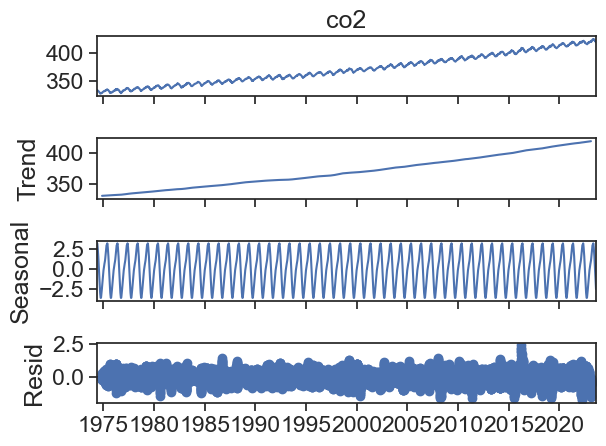
\includegraphics{basics/example_files/figure-pdf/cell-5-output-1.png}

\section{first plot, v2.0}\label{first-plot-v2.0}

The dates in the x-label are not great. Let's try to make them prettier.

We need to import a few more packages first.

\begin{Shaded}
\begin{Highlighting}[]
\ImportTok{import}\NormalTok{ matplotlib.dates }\ImportTok{as}\NormalTok{ mdates}
\ImportTok{from}\NormalTok{ matplotlib.dates }\ImportTok{import}\NormalTok{ DateFormatter}
\ImportTok{from}\NormalTok{ pandas.plotting }\ImportTok{import}\NormalTok{ register\_matplotlib\_converters}
\NormalTok{register\_matplotlib\_converters()  }\CommentTok{\# datetime converter for a matplotlib}
\end{Highlighting}
\end{Shaded}

Now let's replot.

\begin{Shaded}
\begin{Highlighting}[]
\CommentTok{\# \%matplotlib widget}
\CommentTok{\# uncomment the above line if you want dynamic control of the figure when using VSCode}
\NormalTok{fig, (ax1, ax2) }\OperatorTok{=}\NormalTok{ plt.subplots(}\DecValTok{1}\NormalTok{, }\DecValTok{2}\NormalTok{,  }\CommentTok{\# 1 row, 2 columns}
\NormalTok{                               figsize}\OperatorTok{=}\NormalTok{(}\DecValTok{8}\NormalTok{,}\DecValTok{5}\NormalTok{)  }\CommentTok{\# width, height, in inches}
\NormalTok{                               )}
\CommentTok{\# left panel}
\NormalTok{ax1.plot(df[}\StringTok{\textquotesingle{}average\textquotesingle{}}\NormalTok{], color}\OperatorTok{=}\StringTok{"black"}\NormalTok{)}
\NormalTok{ax1.plot(df.loc[}\StringTok{\textquotesingle{}2010{-}01{-}01\textquotesingle{}}\NormalTok{:}\StringTok{\textquotesingle{}2011{-}12{-}31\textquotesingle{}}\NormalTok{,}\StringTok{\textquotesingle{}average\textquotesingle{}}\NormalTok{], color}\OperatorTok{=}\StringTok{"magenta"}\NormalTok{)}
\NormalTok{ax1.}\BuiltInTok{set}\NormalTok{(xlabel}\OperatorTok{=}\StringTok{"date"}\NormalTok{,}
\NormalTok{       ylabel}\OperatorTok{=}\VerbatimStringTok{r"CO$\_2$ concentration (ppm)"}\NormalTok{,}
\NormalTok{       title}\OperatorTok{=}\StringTok{"long term"}\NormalTok{)}\OperatorTok{;}
\CommentTok{\# right panel}
\NormalTok{ax2.plot(df.loc[}\StringTok{\textquotesingle{}2010{-}01{-}01\textquotesingle{}}\NormalTok{:}\StringTok{\textquotesingle{}2011{-}12{-}31\textquotesingle{}}\NormalTok{,}\StringTok{\textquotesingle{}average\textquotesingle{}}\NormalTok{], color}\OperatorTok{=}\StringTok{"magenta"}\NormalTok{)}
\NormalTok{ax2.}\BuiltInTok{set}\NormalTok{(xlabel}\OperatorTok{=}\StringTok{"date"}\NormalTok{,}
\NormalTok{        ylabel}\OperatorTok{=}\VerbatimStringTok{r"CO$\_2$ concentration (ppm)"}\NormalTok{,}
\NormalTok{        ylim}\OperatorTok{=}\NormalTok{[}\DecValTok{385}\NormalTok{, }\DecValTok{400}\NormalTok{],  }\CommentTok{\# choose y limits}
\NormalTok{        yticks}\OperatorTok{=}\NormalTok{np.arange(}\DecValTok{385}\NormalTok{, }\DecValTok{401}\NormalTok{, }\DecValTok{5}\NormalTok{),  }\CommentTok{\# choose ticks}
\NormalTok{        title}\OperatorTok{=}\StringTok{"years 2010{-}{-}2011"}\NormalTok{)}\OperatorTok{;}
\CommentTok{\# put ticks and label on the right for ax2}
\NormalTok{ax2.yaxis.tick\_right()}
\NormalTok{ax2.yaxis.set\_label\_position(}\StringTok{"right"}\NormalTok{)}
\CommentTok{\# title above both panels}
\NormalTok{fig.suptitle(}\StringTok{"Mauna Loa Observatory"}\NormalTok{, y}\OperatorTok{=}\FloatTok{1.00}\NormalTok{)}

\NormalTok{locator }\OperatorTok{=}\NormalTok{ mdates.AutoDateLocator(minticks}\OperatorTok{=}\DecValTok{3}\NormalTok{, maxticks}\OperatorTok{=}\DecValTok{5}\NormalTok{)}
\NormalTok{formatter }\OperatorTok{=}\NormalTok{ mdates.ConciseDateFormatter(locator)}
\NormalTok{ax1.xaxis.set\_major\_locator(locator)}
\NormalTok{ax1.xaxis.set\_major\_formatter(formatter)}

\NormalTok{locator }\OperatorTok{=}\NormalTok{ mdates.AutoDateLocator(minticks}\OperatorTok{=}\DecValTok{4}\NormalTok{, maxticks}\OperatorTok{=}\DecValTok{5}\NormalTok{)}
\NormalTok{formatter }\OperatorTok{=}\NormalTok{ mdates.ConciseDateFormatter(locator)}
\NormalTok{ax2.xaxis.set\_major\_locator(locator)}
\NormalTok{ax2.xaxis.set\_major\_formatter(formatter)}

\NormalTok{ax1.annotate(}
    \StringTok{"2010/11"}\NormalTok{,}
\NormalTok{    xy}\OperatorTok{=}\NormalTok{(}\StringTok{\textquotesingle{}2011{-}12{-}25\textquotesingle{}}\NormalTok{, }\DecValTok{389}\NormalTok{),  xycoords}\OperatorTok{=}\StringTok{\textquotesingle{}data\textquotesingle{}}\NormalTok{,}
\NormalTok{    xytext}\OperatorTok{=}\NormalTok{(}\OperatorTok{{-}}\DecValTok{10}\NormalTok{, }\OperatorTok{{-}}\DecValTok{80}\NormalTok{), textcoords}\OperatorTok{=}\StringTok{\textquotesingle{}offset points\textquotesingle{}}\NormalTok{,}
\NormalTok{    arrowprops}\OperatorTok{=}\BuiltInTok{dict}\NormalTok{(arrowstyle}\OperatorTok{=}\StringTok{"{-}\textgreater{}"}\NormalTok{,}
\NormalTok{                    color}\OperatorTok{=}\StringTok{"black"}\NormalTok{,}
\NormalTok{                    connectionstyle}\OperatorTok{=}\StringTok{"arc3,rad=0.2"}\NormalTok{))}
\NormalTok{fig.savefig(}\StringTok{"CO2{-}graph.png"}\NormalTok{, dpi}\OperatorTok{=}\DecValTok{300}\NormalTok{)}
\end{Highlighting}
\end{Shaded}

\begin{verbatim}
/var/folders/hc/jhnmlst937d27zzq9fhfks780000gn/T/ipykernel_10652/850389963.py:42: UserWarning: AutoDateLocator was unable to pick an appropriate interval for this date range. It may be necessary to add an interval value to the AutoDateLocator's intervald dictionary. Defaulting to 6.
  fig.savefig("CO2-graph.png", dpi=300)
/opt/anaconda3/lib/python3.9/site-packages/IPython/core/pylabtools.py:151: UserWarning: AutoDateLocator was unable to pick an appropriate interval for this date range. It may be necessary to add an interval value to the AutoDateLocator's intervald dictionary. Defaulting to 6.
  fig.canvas.print_figure(bytes_io, **kw)
\end{verbatim}

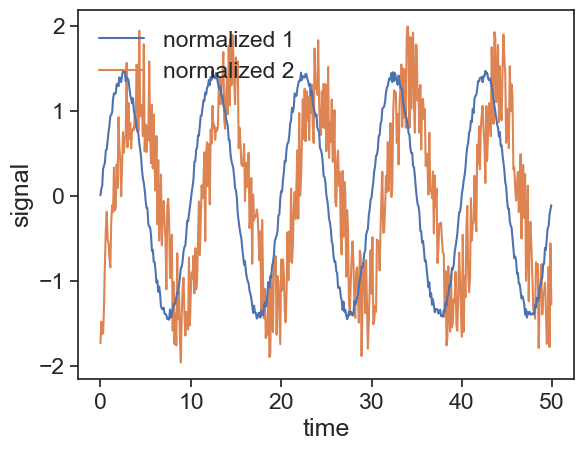
\includegraphics{basics/example_files/figure-pdf/cell-7-output-2.png}

The dates on the horizontal axis are determined thus:

\begin{enumerate}
\def\labelenumi{\arabic{enumi}.}
\tightlist
\item
  \texttt{locator\ =\ mdates.AutoDateLocator(minticks=3,\ maxticks=5)}\strut \\
  This deremines the location of the ticks (between 3 and 5 ticks,
  whatever ``works best'')
\item
  \texttt{ax1.xaxis.set\_major\_locator(locator)}\strut \\
  This actually puts the ticks in the positions determined above
\item
  \texttt{formatter\ =\ mdates.ConciseDateFormatter(locator)}\strut \\
  This says that the labels will be placed at the locations determined
  in 1.
\item
  \texttt{ax1.xaxis.set\_major\_formatter(formatter)}\strut \\
  Finally, labels are written down
\end{enumerate}

The arrow is placed in the graph using \texttt{annotate}. It has a
tricky syntax and a million options. Read
\href{https://jakevdp.github.io/PythonDataScienceHandbook/04.09-text-and-annotation.html\#Arrows-and-Annotation}{Jake
VanderPlas's} excellent examples to learn more.

\section{modifications}\label{modifications}

Let's change a lot of plotting options to see how things could be
different.

\begin{Shaded}
\begin{Highlighting}[]
\NormalTok{sns.}\BuiltInTok{set}\NormalTok{(style}\OperatorTok{=}\StringTok{"darkgrid"}\NormalTok{)}
\NormalTok{sns.set\_context(}\StringTok{"notebook"}\NormalTok{)}

\CommentTok{\# \%matplotlib widget}
\CommentTok{\# uncomment the above line if you want dynamic control of the figure when using VSCode}
\NormalTok{fig, (ax1, ax2) }\OperatorTok{=}\NormalTok{ plt.subplots(}\DecValTok{1}\NormalTok{, }\DecValTok{2}\NormalTok{,  }\CommentTok{\# 1 row, 2 columns}
\NormalTok{                               figsize}\OperatorTok{=}\NormalTok{(}\DecValTok{8}\NormalTok{,}\DecValTok{4}\NormalTok{)  }\CommentTok{\# width, height, in inches}
\NormalTok{                               )}
\CommentTok{\# left panel}
\NormalTok{ax1.plot(df[}\StringTok{\textquotesingle{}average\textquotesingle{}}\NormalTok{], color}\OperatorTok{=}\StringTok{"tab:blue"}\NormalTok{)}
\NormalTok{ax1.plot(df.loc[}\StringTok{\textquotesingle{}2010{-}01{-}01\textquotesingle{}}\NormalTok{:}\StringTok{\textquotesingle{}2011{-}12{-}31\textquotesingle{}}\NormalTok{,}\StringTok{\textquotesingle{}average\textquotesingle{}}\NormalTok{], color}\OperatorTok{=}\StringTok{"tab:orange"}\NormalTok{)}
\NormalTok{ax1.}\BuiltInTok{set}\NormalTok{(xlabel}\OperatorTok{=}\StringTok{"date"}\NormalTok{,}
\NormalTok{       ylabel}\OperatorTok{=}\VerbatimStringTok{r"CO$\_2$ concentration (ppm)"}\NormalTok{,}
\NormalTok{       title}\OperatorTok{=}\StringTok{"long term"}\NormalTok{)}\OperatorTok{;}
\CommentTok{\# right panel}
\NormalTok{ax2.plot(df.loc[}\StringTok{\textquotesingle{}2010{-}01{-}01\textquotesingle{}}\NormalTok{:}\StringTok{\textquotesingle{}2011{-}12{-}31\textquotesingle{}}\NormalTok{,}\StringTok{\textquotesingle{}average\textquotesingle{}}\NormalTok{], color}\OperatorTok{=}\StringTok{"tab:orange"}\NormalTok{)}
\NormalTok{ax2.}\BuiltInTok{set}\NormalTok{(xlabel}\OperatorTok{=}\StringTok{"date"}\NormalTok{,}
\NormalTok{        ylim}\OperatorTok{=}\NormalTok{[}\DecValTok{385}\NormalTok{, }\DecValTok{400}\NormalTok{],  }\CommentTok{\# choose y limits}
\NormalTok{        yticks}\OperatorTok{=}\NormalTok{np.arange(}\DecValTok{385}\NormalTok{, }\DecValTok{401}\NormalTok{, }\DecValTok{5}\NormalTok{),  }\CommentTok{\# choose ticks}
\NormalTok{        title}\OperatorTok{=}\StringTok{"years 2010{-}{-}2011"}\NormalTok{)}\OperatorTok{;}
\CommentTok{\# title above both panels}
\NormalTok{fig.suptitle(}\StringTok{"Mauna Loa Observatory"}\NormalTok{, y}\OperatorTok{=}\FloatTok{1.00}\NormalTok{)}

\NormalTok{locator }\OperatorTok{=}\NormalTok{ mdates.AutoDateLocator(minticks}\OperatorTok{=}\DecValTok{3}\NormalTok{, maxticks}\OperatorTok{=}\DecValTok{5}\NormalTok{)}
\NormalTok{formatter }\OperatorTok{=}\NormalTok{ mdates.ConciseDateFormatter(locator)}
\NormalTok{ax1.xaxis.set\_major\_locator(locator)}
\NormalTok{ax1.xaxis.set\_major\_formatter(formatter)}

\NormalTok{locator }\OperatorTok{=}\NormalTok{ mdates.AutoDateLocator(minticks}\OperatorTok{=}\DecValTok{5}\NormalTok{, maxticks}\OperatorTok{=}\DecValTok{8}\NormalTok{)}
\NormalTok{formatter }\OperatorTok{=}\NormalTok{ mdates.ConciseDateFormatter(locator)}
\NormalTok{ax2.xaxis.set\_major\_locator(locator)}
\NormalTok{ax2.xaxis.set\_major\_formatter(formatter)}

\NormalTok{ax1.annotate(}
    \StringTok{"2010/11"}\NormalTok{,}
\NormalTok{    xy}\OperatorTok{=}\NormalTok{(}\StringTok{\textquotesingle{}2010{-}12{-}25\textquotesingle{}}\NormalTok{, }\DecValTok{395}\NormalTok{),  xycoords}\OperatorTok{=}\StringTok{\textquotesingle{}data\textquotesingle{}}\NormalTok{,}
\NormalTok{    xytext}\OperatorTok{=}\NormalTok{(}\OperatorTok{{-}}\DecValTok{100}\NormalTok{, }\DecValTok{40}\NormalTok{), textcoords}\OperatorTok{=}\StringTok{\textquotesingle{}offset points\textquotesingle{}}\NormalTok{,}
\NormalTok{    bbox}\OperatorTok{=}\BuiltInTok{dict}\NormalTok{(boxstyle}\OperatorTok{=}\StringTok{"round4,pad=.5"}\NormalTok{, fc}\OperatorTok{=}\StringTok{"white"}\NormalTok{),}
\NormalTok{    arrowprops}\OperatorTok{=}\BuiltInTok{dict}\NormalTok{(arrowstyle}\OperatorTok{=}\StringTok{"{-}\textgreater{}"}\NormalTok{,}
\NormalTok{                    color}\OperatorTok{=}\StringTok{"black"}\NormalTok{,}
\NormalTok{                    connectionstyle}\OperatorTok{=}\StringTok{"angle,angleA=0,angleB={-}90,rad=40"}\NormalTok{))}
\end{Highlighting}
\end{Shaded}

\begin{verbatim}
Text(-100, 40, '2010/11')
\end{verbatim}

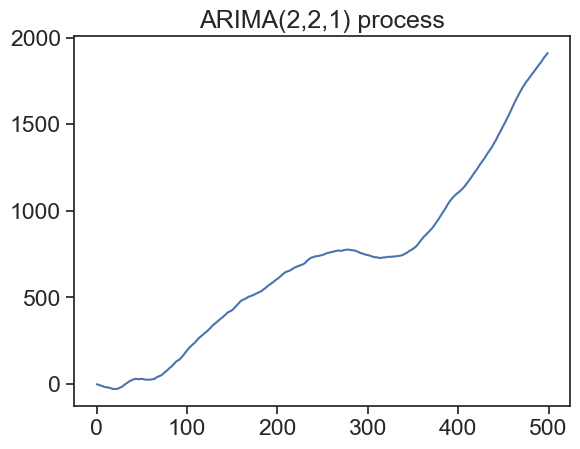
\includegraphics{basics/example_files/figure-pdf/cell-8-output-2.png}

The main changes were:

\begin{enumerate}
\def\labelenumi{\arabic{enumi}.}
\tightlist
\item
  Using the Seaborn package, we changed the fontsize and the overall
  plot style.
  \href{https://seaborn.pydata.org/tutorial/aesthetics.html}{Read
  more}.\\
  \texttt{sns.set(style="darkgrid")}\strut \\
  \texttt{sns.set\_context("notebook")}
\item
  We changed the colors of the lineplots. To know what colors exist,
  \href{https://matplotlib.org/stable/gallery/color/named_colors.html}{click
  here}.
\item
  The arrow annotation has a different style.
  \href{https://jakevdp.github.io/PythonDataScienceHandbook/04.09-text-and-annotation.html\#Arrows-and-Annotation}{Read
  more}.
\end{enumerate}

\section{playing with the code}\label{playing-with-the-code}

I encourage you to play with the code you just ran. An easy way of
learning what each line does is to comment something out and see what
changes in the output you see. If you feel brave, try to modify the code
a little bit.




\end{document}
